%                                                                 aa.dem
% AA vers. 9.1, LaTeX class for Astronomy & Astrophysics
% demonstration file
%                                                       (c) EDP Sciences
%-----------------------------------------------------------------------
%
%\documentclass[referee]{aa} % for a referee version
%\documentclass[onecolumn]{aa} % for a paper on 1 column  
%\documentclass[longauth]{aa} % for the long lists of affiliations 
%\documentclass[letter]{aa} % for the letters 
%\documentclass[bibyear]{aa} % if the references are not structured 
%                              according to the author-year natbib style

%
\documentclass{aa}  

%
\usepackage{graphicx}
%%%%%%%%%%%%%%%%%%%%%%%%%%%%%%%%%%%%%%%%
\usepackage{txfonts}
%%%%%%%%%%%%%%%%%%%%%%%%%%%%%%%%%%%%%%%%
%\usepackage[options]{hyperref}
% To add links in your PDF file, use the package "hyperref"
% with options according to your LaTeX or PDFLaTeX drivers.
\usepackage[colorlinks=true,citecolor=blue,linkcolor=blue]{hyperref}
% To add links in your PDF file, use the package "hyperref"
% with options according to your LaTeX or PDFLaTeX drivers.
%
\usepackage{natbib}
\bibpunct{(}{)}{;}{a}{}{,} % to follow the A&A style
%\usepackage{enumitem}
\usepackage{bm}
\usepackage{upgreek}
\usepackage[dvipsnames]{xcolor}
\usepackage{amsmath}    % Advanced maths commands
%\usepackage{amssymb}
%

\newcommand{\nlens}{20}

\begin{document} 


   \title{Lens models of galaxy--galaxy strong lenses}

   \subtitle{}

   \author{BDLensing team
          \inst{1}
          \and
          C. Ptolemy\inst{2}\fnmsep\thanks{Just to show the usage
          of the elements in the author field}
          }

   \institute{Institute for Astronomy (IfA), University of Vienna,
              T\"urkenschanzstrasse 17, A-1180 Vienna\\
              \email{wuchterl@amok.ast.univie.ac.at}
         \and
             University of Alexandria, Department of Geography, ...\\
             \email{c.ptolemy@hipparch.uheaven.space}
             \thanks{The university of heaven temporarily does not
                     accept e-mails}
             }

   \date{Received September 15, 1996; accepted March 16, 1997}

% \abstract{}{}{}{}{} 
% 5 {} token are mandatory
 
  \abstract
  % context heading (optional)
  % {} leave it empty if necessary  
   {To investigate the physical nature of the `nuc\-leated instability' of
   proto giant planets, the stability of layers
   in static, radiative gas spheres is analysed on the basis of Baker's
   standard one-zone model.}
  % aims heading (mandatory)
   {It is shown that stability
   depends only upon the equations of state, the opacities and the local
   thermodynamic state in the layer. Stability and instability can
   therefore be expressed in the form of stability equations of state
   which are universal for a given composition.}
  % methods heading (mandatory)
   {The stability equations of state are
   calculated for solar composition and are displayed in the domain
   $-14 \leq \lg \rho / \mathrm{[g\, cm^{-3}]} \leq 0 $,
   $ 8.8 \leq \lg e / \mathrm{[erg\, g^{-1}]} \leq 17.7$. These displays
   may be
   used to determine the one-zone stability of layers in stellar
   or planetary structure models by directly reading off the value of
   the stability equations for the thermodynamic state of these layers,
   specified
   by state quantities as density $\rho$, temperature $T$ or
   specific internal energy $e$.
   Regions of instability in the $(\rho,e)$-plane are described
   and related to the underlying microphysical processes.}
  % results heading (mandatory)
   {Vibrational instability is found to be a common phenomenon
   at temperatures lower than the second He ionisation
   zone. The $\kappa$-mechanism is widespread under `cool'
   conditions.}
  % conclusions heading (optional), leave it empty if necessary 
   {}

   \keywords{giant planet formation --
                $\kappa$-mechanism --
                stability of gas spheres
               }

   \maketitle
%
%-------------------------------------------------------------------

\section{Introduction}

Strong gravitational lensing is the phenomenon of forming multiple images from a background source due to the gravitational bending of light path by a massive foreground deflector, such as a galaxy, galaxy group, or cluster. As a result, strong lensing systems are powerful probes of the mass distribution of the foreground deflector \citep[see][for a review on strong lensing by galaxies]{Shajib22}.

Whereas the observed light traces the stars in a lensing galaxy, strong lensing traces the total matter distribution, including dark and baryonic components. As a result, strong lensing can be used to study the relative alignment between dark matter and stars. Any detected offset between these two components can indicate self-interaction in the dark matter particles \citep{Harvey14, Kahlhoefer14, Robertson17}. In the $\Lambda$ cold dark matter ($\Lambda$CDM) cosmology -- the current paradigm to describe our Universe -- the EAGLE simulation predicts no significant offset $\sim$200 pc, regardless of the galaxy being a field galaxy or a cluster member \citep{Schaller15}. Although a recent merger can lead to an offset between the dark matter and stars, these systems are statistically very rare \citep{Schaller15}. On the observational front, only one system has been observed with an offset much larger than this prediction ($1.72\pm 0.42$ kpc), where the deflector consists of two merging galaxies  \citep[][]{Shu16}. %Although there was an initial report of a similar offset for a cluster-member galaxy in Abell 3827 \citep{Williams11, Massey15}, the offset was ruled out with more data \citep{Massey18}.
\citet{Shajib19} find a root-mean-square (RMS) offset in a sample of 13 strong lenses to be 0\farcs04 (i.e., $\sim$200 pc at z$\sim$0.5) excluding three outliers, one of which has two comparable-mass deflectors potentially residing in the same parent halo. Similarly, \citet{Shajib21} constrained a 68 percent upper limit of 218$\pm$19 pc from a sample of 23 galaxy--galaxy lenses.

The misalignment between the mass and light distributions can also be traced using the position angles of the major axes of the elliptical galaxies, which are the most common type of deflectors at the galaxy scale. Previous studies mostly found tight alignment within $\sim$10$\degr$ \citep{Keeton98b, Kochanek02, Treu09, Gavazzi12, Sluse12, Bruderer16, Shajib19, Shajib21}, with higher misalignments are accompanied by large ``external'' shear magnitude, although the vice versa is not necessary. The accompaniment of a large ``external'' shear with a large misalignment can be interpreted as systems in a crowded environment that are not yet dynamically relaxed, as they can have stellar orbits misaligned with the underlying dark matter distribution. Simulations found highly misaligned orbits in isolated systems to be unstable and rare \citep{Heiligman79, Martinet88, Adams07, Debattista15}. However, this interpretation treats ``external'' shear as originating purely from nearby line-of-sight galaxies external to the central deflector. Interestingly, \citet{Etherington23} suggested that this ``external'' shear is not purely of external origin and can arise from the inadequacy of the mass model for lensing galaxy in capturing all of its angular complexity \citep[for example, boxy/discyness, ellipticity gradient, isophotal twists;][]{VandeVyvere22, VandeVyvere22b}. This suggestion from \citet{Etherington23} makes the explanation of high misalignment as stemming from interaction with a crowded environment less favorable.

In this paper, we investigate the alignment between the mass and light using a sample of \nlens\  galaxies. We present power-law mass models of these systems based on \textit{Hubble Space Telescope} (\textit{HST}) imaging data. Using our lens models, we perform two experiments. First, we check if there is a difference in the mass and light offset between isolated and non-isolated galaxies and test the prediction of no difference from the EAGLE simulation. Second, we investigate if the misalignment between light and mass major axes directly correlates with the local galaxy density. This second experiment more directly tests the hypothesis that galaxies with stellar orbits misaligned with dark matter live in crowded environments without adopting the ``external'' shear as a measure of a crowded environment.

This paper is organized as follows. In Section \ref{sec:data}, we describe our lens sample and the \textit{HST} data we model. Then in Section \ref{sec:modeling_method}, we describe our lens modelling method. We present our results in Section \ref{sec:result}. Finally, we discuss our result and conclude the paper in Section \ref{sec:discussion}. Throughout the paper, we adopt a flat $\Lambda$CDM cosmology as the fiducial cosmology with $H_0= 70$ km s$^{-1}$ Mpc$^{-1}$ and $\Omega_{\rm m} = 0.3$.

\section{Data} \label{sec:data}
Our sample comprises of 20 strong lensing systems. All of the strong galaxy-galaxy lensing candidates discovered in the Dark Energy Spectroscopic Instrument (DESI) Legacy Imaging Surveys, Data Release 7, using a deep neural network. Each system in our sample has multiple lensed images. In this section, we first describe the high-resolution imaging data obtained through HST. We then provide a brief overview of the lens systems in the sample.


\subsection{\textit{HST} imaging} 

Images of the lenses were obtained using the HST Wide Field Camera 3 (WFC3) in a specific filter: F140W in the infrared (IR) channel. The wide F140W filter covers the gap between the J and H bands that is inaccessible from the ground. 

% example https://arxiv.org/pdf/2008.11724.pdf and https://arxiv.org/pdf/1807.09278.pdf

\subsection{Description of special systems (can be finalized later)}

% example in https://arxiv.org/pdf/1807.09278.pdf

\begin{figure*}
	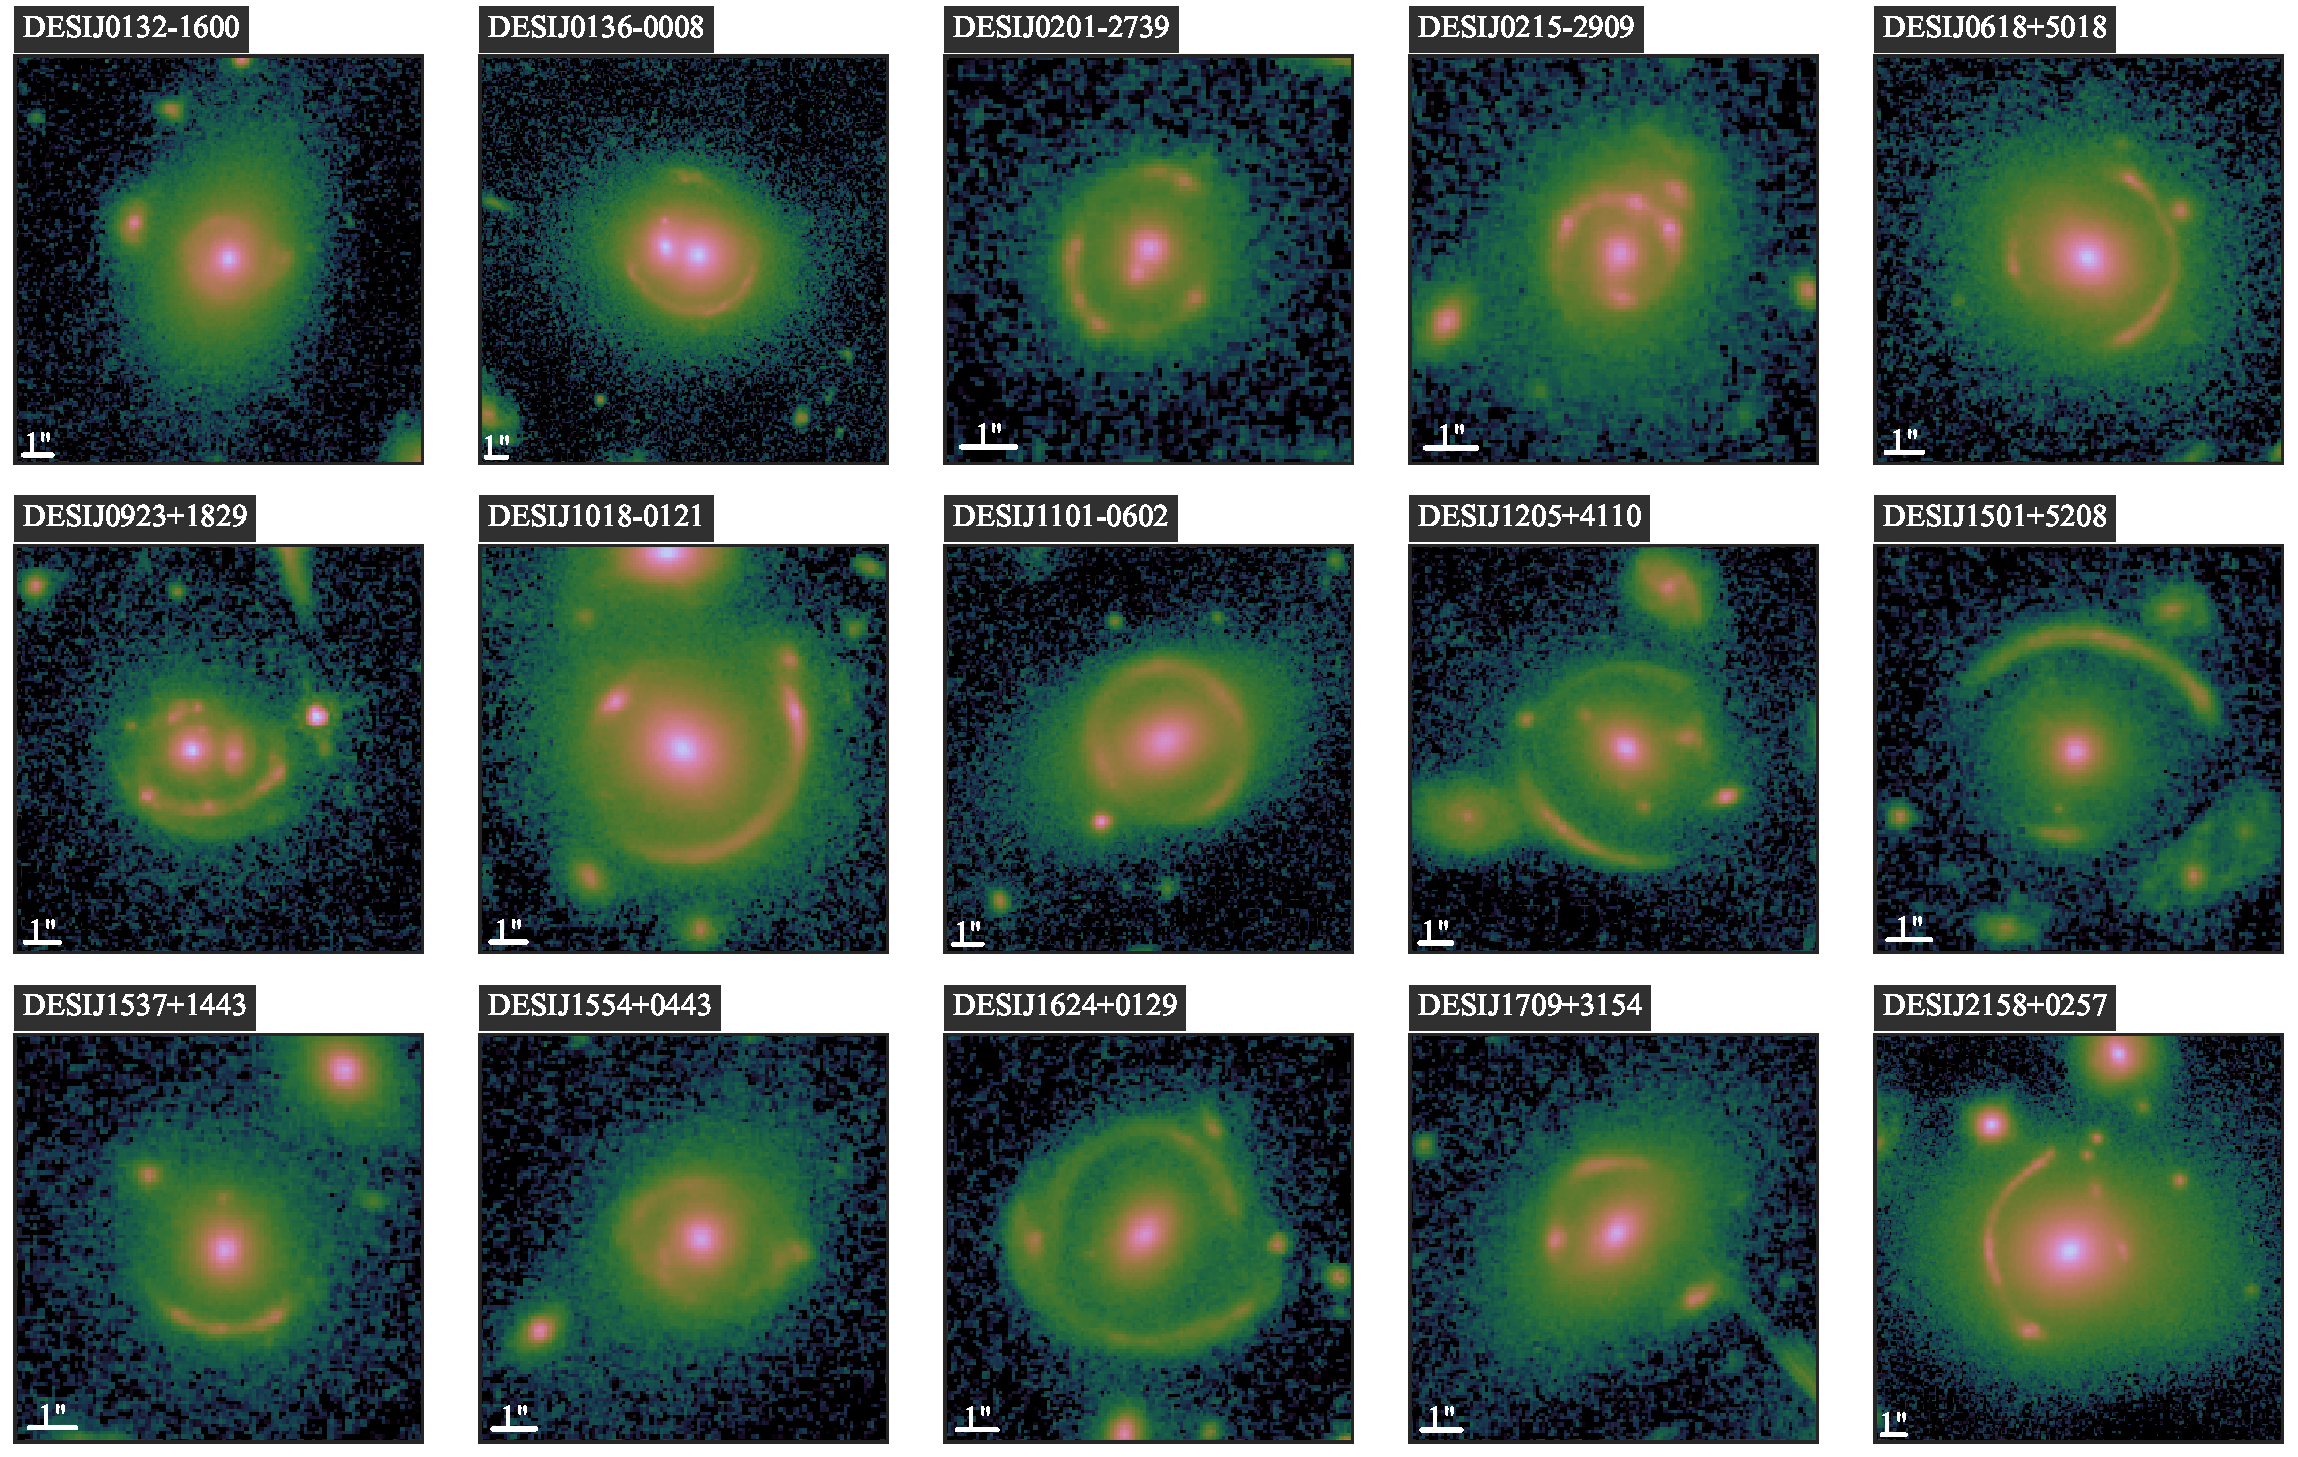
\includegraphics[width=\textwidth]{figures/lens_montage.pdf}
	\caption{\label{fig:montage}
	Montage of all the lens systems.
	}
\end{figure*}

\subsubsection{DESIJ0132$-$1600}
% Anik's Model

The central deflector in this system produces a lensing effect resembling a ring shape. Except for one conspicuous large object to the left of the lensing system, all other noticeable objects have been masked out. When modeling the source light of the system, we solely utilized the SHAPELETS profile, while the lens mass and light were modeled using EPL and S\'ersic profiles, respectively.

\subsubsection{DESIJ0136$-$0008}
% Akbar's Model

This system has two lensing galaxies of comparable sizes within the Einstein radius. Another smaller object also exists within the Einstein radius, which is potentially a third-member galaxy within this group. We model the larger galaxy on the west as the main deflector. We also explicitly modeled the mass profile of the large companion with a SIE model. However, we assumed the lensing effect of the potential third group member is negligible, given its relatively smaller size and not being in close proximity to the arcs, and masked over its light. We also noticed some prominent residual in between the two largest galaxies that the smooth S\'ersic profiles were not adequate to describe. This non-smooth structure may potentially arise if these two galaxies are interacting or merging. We also masked out a small strip in between the galaxies to exclude this non-smooth structure in the light distribution (Figure \ref{fig:lens_models}).


\subsubsection{DESIJ0201$-$2739}
% Rafee's Model

In this system, an elliptical lensing effect is evident, showing a major central component and a minor one. We attribute the primary lensing arc to the significant central galaxy, while considering the contribution of the minor central galaxy using a SIE mass profile. To encompass both companions, we adopted a double S\'ersic  profile to model the central galaxy and single S\'ersic  profile to model the other one. To focus solely on the lensing contribution, we masked out a small source on the north-west side of the arc. Ultimately, the model generated a comprehensive elliptical ring for the system.

\subsubsection{DESIJ0215$-$2909}
% Milli's Model

At first glance, this lensing system appears to exhibit a spiral structure. Although it has a resemblance to a quad-system, its notable lensing effect qualifies it as a strong lensing candidate. Prior to modeling, we masked out a blob near the southeast corner and a light structure near the 2 o'clock position. This modeling approach required the introduction of a double SHAPELETS profile to accurately represent the source contribution.

\subsubsection{DESIJ0618$-$5018}
% Nishuti's Model


\subsubsection{DESIJ1018$-$0121}
% Jobair's Model

We assumed the arc spanning from around 2 o'clock position to around 8 o'clock position as the main component of the gravitational lensing arc with a smaller blob at around 10:30 as its counter image. Masking was done by covering non-lensing elements of the image. The system is surrounded by some stars and galaxies which are masked out.

\subsubsection{DESIJ1205$+$4110}
% Robin's Model


\subsubsection{DESIJ1554$+$0443}
% Zareef's Model

In this lensing system, the system itself is relatively small, with a diameter of approximately 4 arcseconds. During modeling, we masked only a blob located near the southeast. Standard mass profiles and light profiles like EPL and S\'ersic  were utilized in this analysis. Two prominent arc features were observed, and following the modeling process, these features formed a complete elliptical ring.

\subsection{DESIJ1501$+$5208}
% Nahid's model

This system exhibits a crescent-shaped major lensing effect, complemented by its counter-image, indicating its candidacy as a strong lensing system. We observed a very faint object near the counter image, but we excluded it from the lensing system during the modeling process. Additionally, several objects located outside the Einstein radius were also masked. Our modeling approach involved the use of the EPL profile for mass and the S\'ersic  profile for light. Despite our efforts, we encountered difficulty in identifying suitable parameters to model certain residual blue features within the Einstein radius. However, these features did not significantly affect the lensing parameters themselves.


\subsubsection{DESIJ1537$+$1443}
% tanver's model

This system prominently displays a strong lensing arc towards the south of the main deflector. The primary gravitational lensing structure extends approximately from the 4 o'clock position to around 8:30 o'clock, accompanied by a smaller blob positioned around the 12 o'clock mark, serving as its corresponding counter image. However, the proximity of the lensing system to another galaxy blob in the northwest necessitated its exclusion through masking during the modeling process. Additionally, a smaller mask was applied close to the 10 o'clock position. We employed standard mass and light profiles to construct the lenses during the modeling phase.

\subsubsection{DESIJ1624$+$0129}
% Imtiaz's model

This system exhibits prominent lensing effects with a well-defined major lensing component and its corresponding counter-image, clearly distinguishable. Our model detected a satellite companion close to the 3 o'clock position, which we addressed using the SIE profile. Additional elements positioned outside the Einstein radius, particularly towards the south and near the 4 o'clock position, were excluded. However, upon completing the modeling process, we identified the need for further masking above the arcs themselves. Although this additional masking did not significantly alter the intended parameters for the lens, it did contribute to the overall system's light.


\subsubsection{DESIJ1709$+$3154}
% tanzilla's model

In this lensing system, three prominent arc features have been observed, modeled using the standard EPL profile for mass and the S\'ersic  profile for light. Additionally, there are some light features in the southeast, identified as diffraction spikes from a nearby large line of sight star. To eliminate these effects, we utilized masking techniques. Furthermore, a very faint object located to the right of the lensing system has also been masked out.

\subsubsection{DESIJ2158$+$0257}
% Fahim's Model

In this system, various objects reside within a densely populated area encompassing the Einstein radius. A significant arc is discernible, formed by the central deflector on the left side with its corresponding counter image on the right. To ensure accurate modeling, we strategically masked two regions within the Einstein radius and several larger nearby objects/stars, excluding contributions from line-of-sight objects and stars with diffraction spikes. Upon closer examination during modeling, we identified additional light sources around the 4 o'clock position. These were present in the observed system but did not appear to be associated with any stars or our lensing system. Consequently, we decided to mask out this particular region. The central lens mass was modeled using the EPL method, while a double S\'ersic profile was employed to model the lens light.


\section{Lens modeling (Method)} \label{sec:modeling_method}

To model the lenses, we used the lens modeling software lenstronomy, available on GitHub1 (Birrer et al. 2015; Bir-rer \& Amara 2018).

\subsection{Lens model ingredients}
We need to pick general models for the lens mass and light to create a method that works well for many lensing systems of different sizes and shapes. These models can be adjusted case by case to fit the specific goals of the investigator. The idea is to make sure the models fit the data nicely while being flexible enough for a wide range of lens systems.

First, we start with basic models for the lens mass, light, and source-light distribution, as explained in Sections 3.1.1 and 3.1.2. Then, we use a Particle Swarm Optimization (PSO) routine in Lenstronomy to find the best fit. After that, we check how well the model fits the data. If it doesn't fit well, we gradually add more details to the model. This might include adding more mass or light details to handle extra things like satellites, complex structures near the Einstein ring, or extra lensed sources.

We also adjust the data, adding or removing bits to make the modeling easier. We run the PSO routine again after each change until the chosen mass and light models give a good fit. Next, we figure out the likelihood of different model parameters using a Markov Chain Monte Carlo (MCMC) routine. The PSO and MCMC routines in Lenstronomy use a package called cosmoHammer, which includes emcee, a smart way to explore different possibilities in the model. This approach helps us model lens systems in a detailed and effective manner.


\subsubsection{Mass profile}
% EPL, external shear 
% example https://arxiv.org/pdf/1807.09278.pdf
\textbf{EPL:} Elliptical Power Law mass profile is given by, 

$$
\kappa\left(x, y\right)=\frac{3-\gamma}{2}\left(\frac{\theta_{\mathrm{E}}}{\sqrt{q x^2+y^2 / q}}\right)^{\gamma-1}
$$

The Elliptical Power Law (EPL) mass profile represents a specific form of the mass distribution used in gravitational lensing studies. It describes the convergence (\(\kappa\)) in terms of the coordinates \(x\) and \(y\) in an elliptical system, where \(x\) and \(y\) represent the Cartesian coordinates on the lens plane, and \(\theta_{\mathrm{E}}\) is the Einstein radius. The parameter \(q\) denotes the axis ratio of the ellipse, representing the elongation or flattening of the mass distribution.
\\
\newline
\textbf{SIE:} Singular Isothermal Ellipsoid (SIE) is given by,

$$
\kappa\left(x, y\right)=\frac{1}{2}\left(\frac{\theta_{\mathrm{E}}}{\sqrt{q x^2+y^2 / q}}\right)
$$

The factor $\frac{1}{2}$ is introduced to scale the convergence appropriately for the SIE model. We used this profile for the fit of the neighboring satellite galaxies.
\\
\newline
\textbf{Shear:} Shear is a measure of the differential stretching or distortion of the images of background sources due to the gravitational lensing effect. It quantifies how much the shapes of background objects are elongated or deformed by the gravitational field of the lensing mass.\\


The pseudo-vector $\vec{\gamma}$=$(\gamma_1, \gamma_2)$ on the lens plane, whose components are
%
\begin{equation}
    \begin{aligned}
        & \gamma_1(\vec{x})=\frac{1}{2}\left(\Psi_{11}-\Psi_{22}\right) \\
        & \gamma_2(\vec{x})=\Psi_{12}=\Psi_{21},
    \end{aligned}
\end{equation}
%
This is called the shear. The eigenvalues of the shear matrix are
$$
\pm \sqrt{\gamma_1^2+\gamma_2^2}= \pm \gamma \text {. }
$$
Thus, there exists a coordinate rotation by an angle $\phi$ such that
$$
\left(\begin{array}{cc}
\gamma_1 & \gamma_2 \\
\gamma_2 & -\gamma_1
\end{array}\right)=\gamma\left(\begin{array}{cc}
\cos 2 \phi & \sin 2 \phi \\
\sin 2 \phi & \cos 2 \phi
\end{array}\right)
$$
\\
\newline 
\textbf{Flexion:} The second order lensing effect can be expressed in terms of the derivatives of the shear (or in terms of the third derivatives of the potential). We can construct the complex quantities
$$
F= F_1 + iF_2 = \left(\gamma_{\mathrm{1,1}} + \gamma_{\mathrm{2,2}}\right) + i\left(\gamma_{\mathrm{2,1}} - \gamma_{\mathrm{1,2}}\right)
$$
$$
G= G_1 + iG_2 = \left(\gamma_{\mathrm{1,1}} - \gamma_{\mathrm{2,2}}\right) + i\left(\gamma_{\mathrm{2,1}} + \gamma_{\mathrm{1,2}}\right)
$$
which are called first and second flexion, respectively. They describe second order distortions of the images of lensed sources. The flexion is responsible for introducing a curvature and other anisotropic distortions
in the images.


\subsubsection{Light profiles}
% Sersic or double sersic for lens galaxy
% Sersic + shapelets for source galaxy
\textbf{SERSIC ELLIPSE:}
We chose the elliptical Sersic function (Sersic 1968) to model the deflector light profile. The Sersic profile is parameterized as

$$
I\left(x_1, y_2\right)=I_{\mathrm{e}} \exp \left[-k\left\{\left(\frac{\sqrt{x^2+y^2 / q_{\mathrm{L}}^2}}{\theta_{\mathrm{eff}}}\right)^{1 / n_{\text {Sersic }}}-1\right\}\right] .
$$

where $R_{\rm eff}$ is the effective radius, $I_e$ is the surface brightness at $R_{\rm eff}$, $q_L$ is axis ratio, $n_{\rm Sersic}$ is the Sérsic index, and $k$ is a normalizing constant so that $R_{\rm eff}$ becomes the half-light radius (Sérsic 1968).
\\
\newline
\textbf{SHAPELETS:}
This profile describes the light distribution of the Source Galaxy. The surface brightness distribution \( S(x, y) \) can be effectively expanded as a sum over shapelet basis functions:
\begin{equation}
    S(x, y) = \sum_{n_x=0}^{\infty} \sum_{n_y=0}^{\infty} c_{n_x,n_y} \bm{\phi}_{n_x,n_y}(x, y)
\end{equation}
The corresponding shapelet coefficients, \( c_{n_x,n_y} \), are determined by performing the overlap integral:
\begin{equation}
    c_{n_x,n_y} = \int \int dx \, dy \, S(x, y) \bm{\phi}_{nx,ny}(x, y)
\end{equation}
Here, \(\bm{\phi}_{nx,ny}(x, y)\) is the two-dimensional Cartesian shapelet function which can be written as the tensor product of two one-dimensional shapelet function, as
\begin{equation}
\begin{aligned}
    \bm{\phi}_{n_x,n_y}(x, y) & \equiv \phi_{n_x}(x) \otimes \phi_{n_y}(y) \\
    &= \beta^{-1} b_{n_x}(\beta^{-1}x) \otimes b_{n_y}(\beta^{-1}y)
\end{aligned}
\end{equation}
Where \( \beta \) represents the characteristic length-scale of the galaxy, and the one-dimensional, dimensionless shapelets function is given by,
\begin{equation}
    b_n(x) \equiv \frac{2^n \sqrt{\pi}}{(2n)!} H_n(x) e^{-\frac{x^2}{2}}
\end{equation}
In this equation, \( n \) is a non-negative integer, and \( H_n(x) \) is a Hermite polynomial of order \( n \).

\subsection{Modelling procedure}

\subsubsection{Initial setup}
% masking, pre-processing of image, psf, intial mass, light profile, source profiles (Rafee)
A cropped section encompassing the lens and its immediate surroundings is chosen to establish an appropriate field-of-view within the entire image. A universally applicable Point Spread Function (PSF) is employed for all the lensing systems. A circular mask, with an appropriate radius, is created to exclusively encompass the deflector-light distribution and associated arcs. In cases where there exists a nearby galaxy or star, these are deliberately masked out, unless a specific decision is made to model the light profile of a satellite or companion galaxy, e.g., for DESIJ0201-2739.

\subsubsection{PSO \& Masking}
%PSO procedure, The elements that were masked, and why, later iterative adjustment of the model (Zobair)
After having an initial mask that keeps the lensed arcs, counterimages, and the other relevant regions of the images exposed, we run the PSO routine in the settings of our initial model assumptions. PSO is the perfect choice for this sort of iterative modeling phase as it is computationally much cheaper than processes like MCMC. PSO (“Particle Swarm Optimization”) mimics the social behavior of a group of living organisms while working together and communicating to find the global optimal values for a set of parameters under certain conditions. The idea was to use PSO as the primary tool while testing different hypotheses regarding the positions of the lensed arcs and counterimages and the complexity of the underlying models. The residual maps were the guides in visualizing the regions where modelings were not close enough and thus steered the process of subsequent model adjustments.
 After settling on a hypothesis about the lensed elements and the necessary complexity of the underlying model, we use MCMC to fit further and calculate the 1$\sigma$ uncertainties of the parameters. \par
The considered sample of the gravitational lenses contains members of different classes of complexities. Some of these were quite simple and the selected base model was sufficient for their modeling while others needed increasingly complex combinations of light and mass profiles. 
The most common case in the addition of complexity was from not being able to remove large residuals in the center which prompted the use of another Sersic light profile on top of the existing one. Another case of multiple occurrences was of satellites near the central lensing galaxy. Masking out was not always possible as it would result in losing the precious lensing data and not being able to include the lensing effect of the satellite itself. In these cases, satellites were modeled using SIE and Sersic ellipse as mass and light profiles respectively. In some cases, the lensing galaxies were in environments congested with unmodeled objects of significant sizes. To account for the gravitational pull of these objects, additional profiles like FLEXION were added. In all of these decision -makings PSO was the touchstone on which we relied. There were also cases where profiles with different parameterizations of the same underlying physical condition were used to facilitate the required level of control. In one of such instances where the model had a high shear value in a certain direction, SHEAR\_GAMMA\_PSI profile was used instead of SHEAR.


\subsubsection{Additional Profiles}
%Extra mass model SIE, extra light profile, add extra shapelets (Robin)
To customize the model for a specific lens system, we needed to add more profiles beyond our initial set. For example: 

SIE: In situations where a nearby satellite has a notable impact on the lensing effects experienced by source galaxies, we introduce a Singular Isothermal Ellipsoid (SIE) profile to characterize its mass distribution. Additionally, a S\'ersic Ellipse (SERSIC ELLIPSE) profile is incorporated to model the light distribution of the satellite. Notably, both profiles are constrained to share the same center.

Second SHAPELETS: In the presence of extra lensed source components, such as blobs or arcs, distinct from the primary source structure near the Einstein ring, additional light profiles (SHAPELETS) are introduced to account for the additional source galaxy. 

Second SERSIC ELLIPSE:

\subsubsection{Ellipticity of light and mass}
%(Rafee)
For some models, the ellipticity of the mass profile was initially unusually higher than the ellipticity of the light profile. So we used a custom log-likelihood function to address this problem. After using the function, the discrepancy in ellipticity was mitigated, aligning more closely with the expected values derived from prior studies.

\subsubsection{Run MCMC}
%(Robin)
Following the completion of the PSO with a viable model, the subsequent step involves the execution of the MCMC. Commencing from the best-fit results obtained through the PSO, this initialization facilitates a rapid convergence of the MCMC chain. Examination of trace plots becomes important in determining the convergence status, where a stable oscillation of walker positions around the median value for all non-linear parameters indicates a successful convergence. The expected behavior of the walker position's oscillation closely resembles a Gaussian distribution, and this characteristic was verified through Corner plots. Finally, a comprehensive reassessment of the model's feasibility was conducted by inspecting the Model Plots, a procedure similar to the approach employed during the PSO process.
% description of PSO, MCMC etc.

\section{Result} \label{sec:result}

\subsection{Lens model parameters}

\begin{figure*}
	\centering
	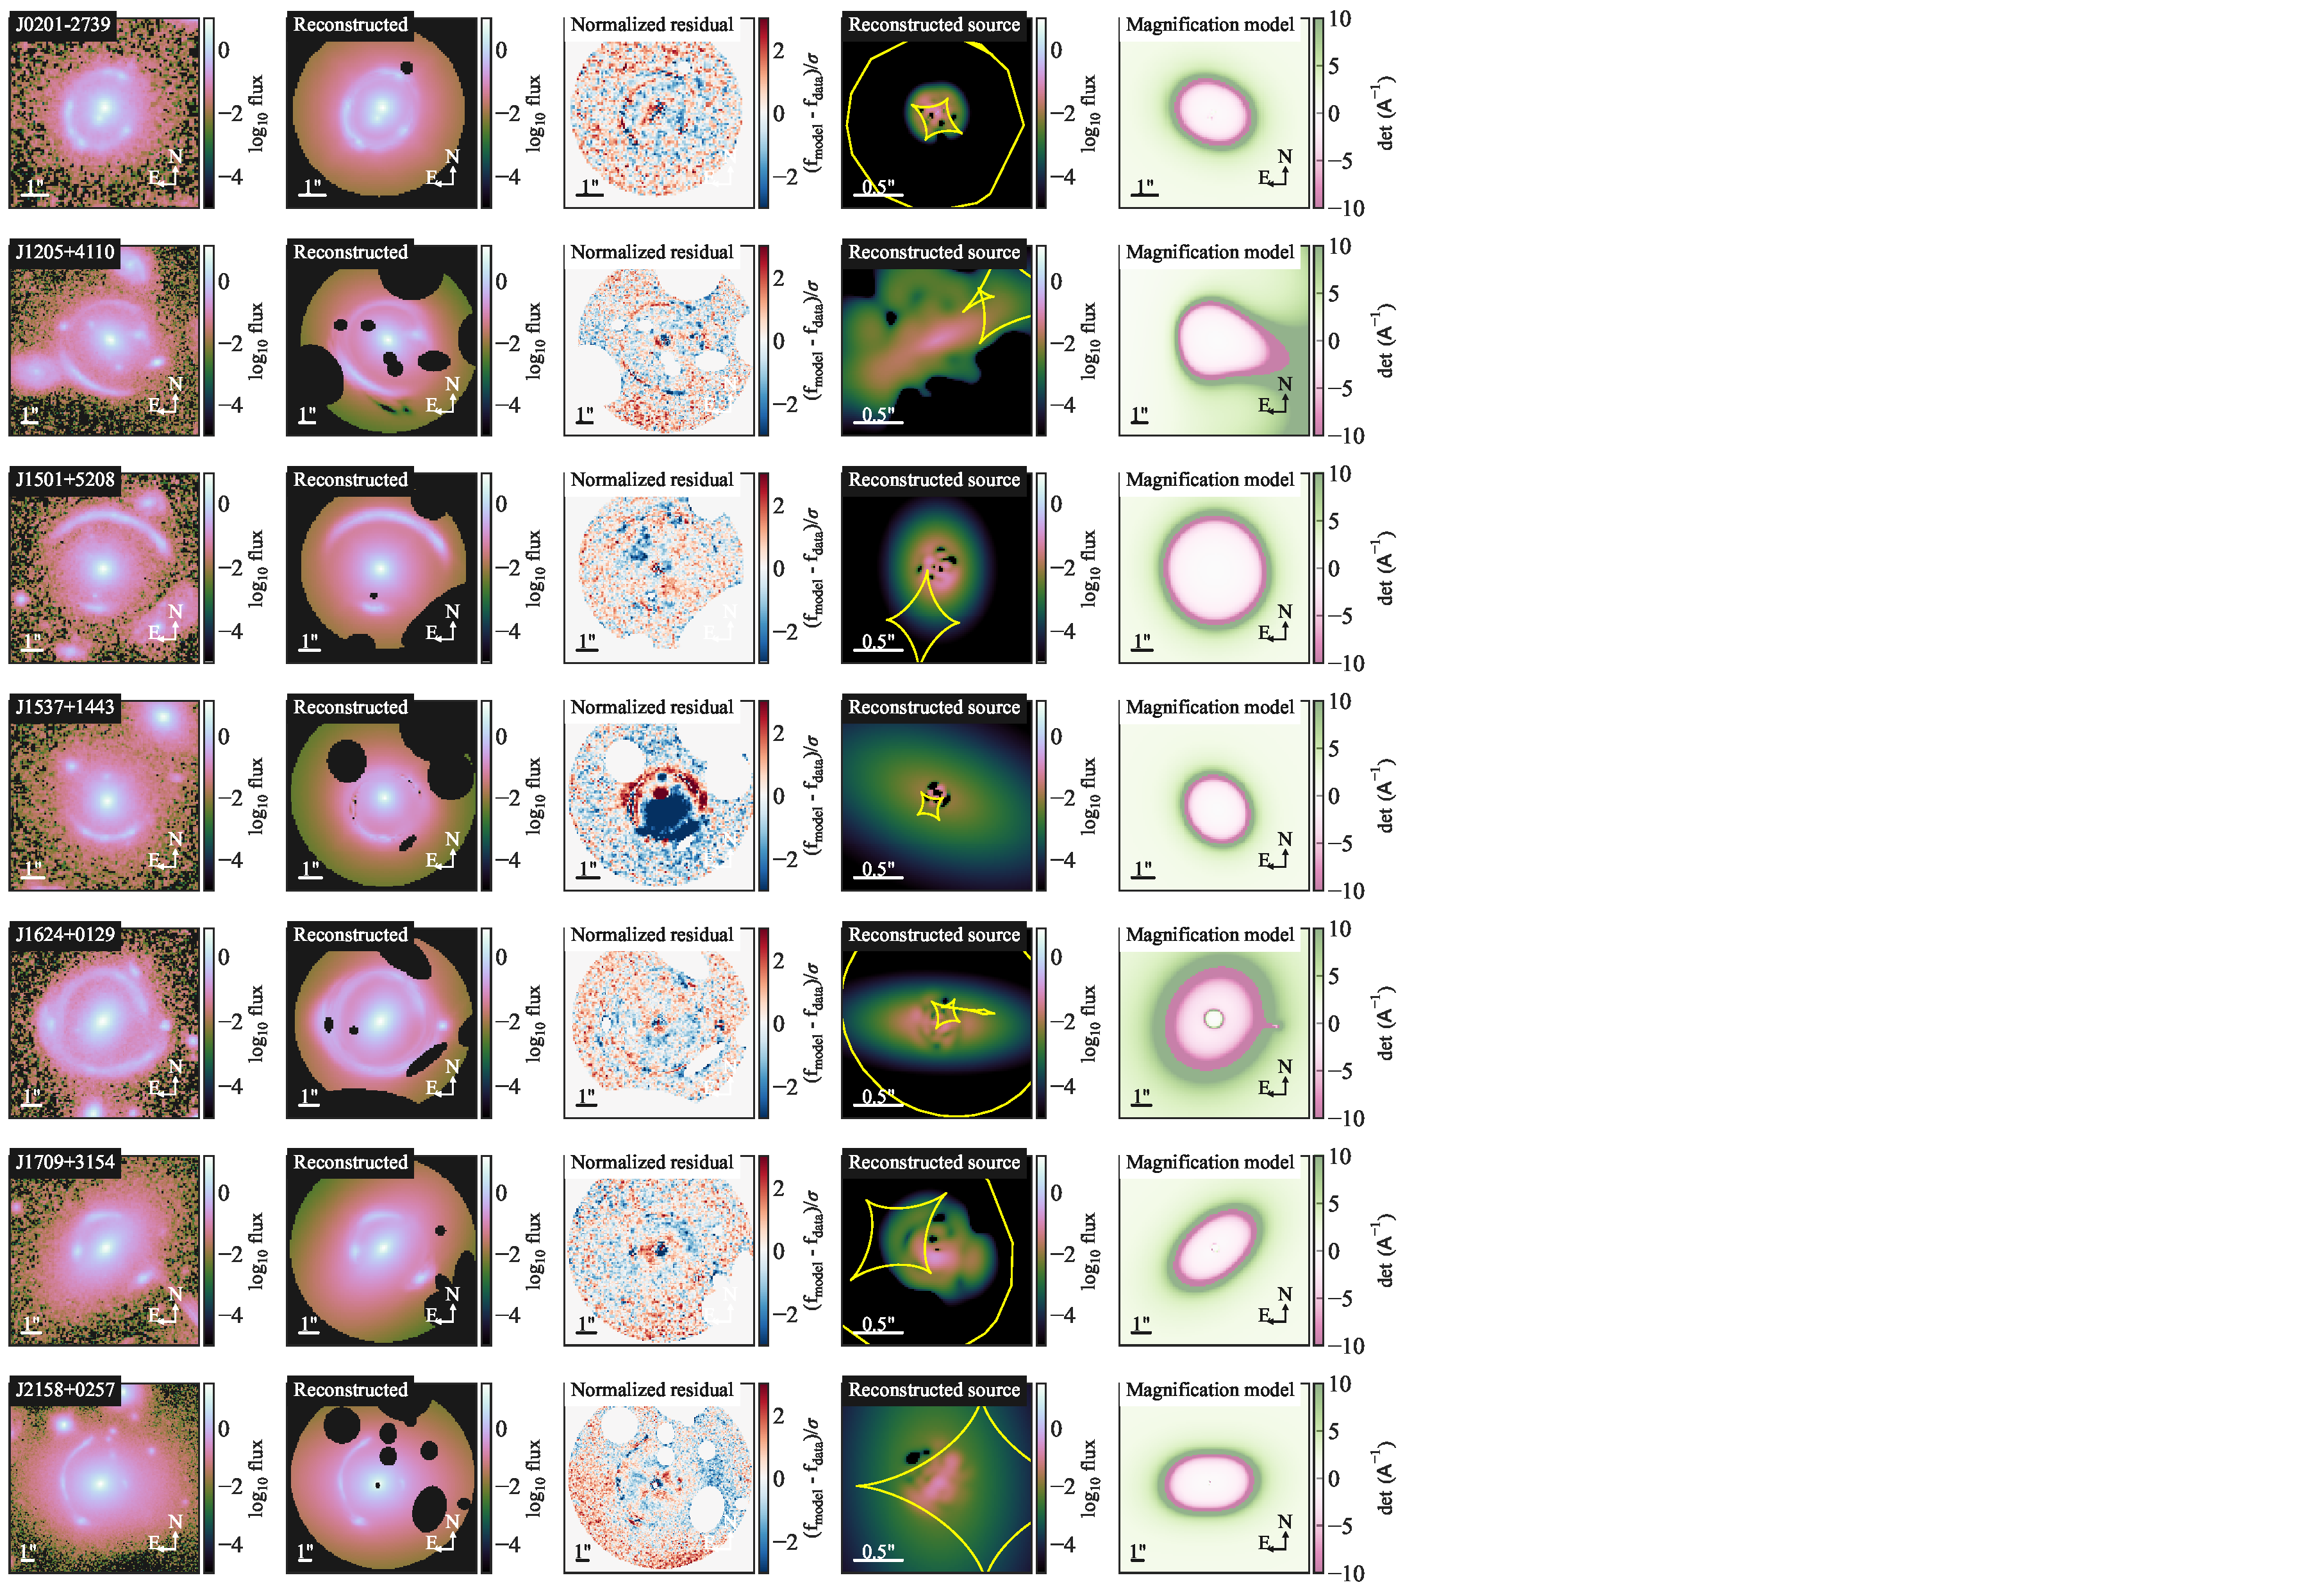
\includegraphics[width=1.55\textwidth]{figures/lens_models.pdf}
	\caption{\label{fig:lens_models}
	Illustration of the lens models for the lens systems in our sample.
	}
\end{figure*}

\renewcommand{\arraystretch}{1.3}
 \begin{table*}
 \caption{Lens model parameters: $\theta_{\rm E}$ is the Einstein radius, $\gamma$ is the logarithmic slope of the mass profile, $q_{\rm m}$ is the mass axis ratio, $\phi_{\rm m}$ is the major axis position angle for mass,  $\gamma_{\rm shear}$ is the residual shear magnitude and $\phi_{\rm shear}$ is the residual shear angle,
 $R_{\rm eff}$ is the effective radius of the light profile,  $q_{\rm L}$ is the light axis ratio, and $\phi_{\rm L}$ is the major axis position angle for light. The angles $\phi_{\rm m}$, $\phi_{\rm shear}$, and $\phi_{\rm L}$ are defined as X of X. The point estimates are the medians of the 1D marginalized posteriors and the 1$\sigma$ uncertainties are obtained from the 16th and 84th percentiles.
\label{table:lens_params}
}
\centering
\begin{tabular}{lccccccccc}
\hline
     System &  $\theta_{\rm E}$ &    $\gamma$ &    $q_\text{m}$ &     $\phi_\text{m}$ &  $\gamma_\text{shear}$  &  $\phi_\text{shear}$  &
     $R_{\rm eff} $ & 
     $q_\text{L}$ & 
     $\phi_\text{L}$
     \\
     & (arcsec) & & &(deg)   & & (deg) & (arcsec) & & (deg) \\
\hline
% column values go into lens_model_param.tex file
J0136$-$0008 &         $2.711_{-0.009}^{+0.008}$ &         $2.01_{-0.02}^{+0.02}$ &         $0.538_{-0.004}^{+0.005}$ &         $70.0_{-0.3}^{+0.3}$ &         $0.134_{-0.003}^{+0.003}$ &         $62.1_{-0.5}^{+0.5}$ &         $0.98 \pm 0.02$ &         $0.900_{-0.001}^{+0.001}$ &         $10.5_{-0.3}^{+0.3}$ \\ 
J0215$-$2909 &         $1.055_{-0.001}^{+0.002}$ &         $1.80_{-0.02}^{+0.01}$ &         $0.717_{-0.005}^{+0.008}$ &         $-88.8_{-0.4}^{+0.5}$ &         $0.011_{-0.003}^{+0.002}$ &         $-81.8_{-4.4}^{+5.6}$ &         $0.92 \pm 0.02$ &         $0.794_{-0.004}^{+0.004}$ &         $-78.9_{-0.7}^{+0.6}$ \\ 
J0618$+$5018 &             $2.265_{-0.001}^{+0.001}$ &             $2.00$ &             $0.726_{-0.002}^{+0.003}$ &             $83.3_{-0.3}^{+0.3}$ &             $0.074_{-0.001}^{+0.001}$ &             $79.1_{-0.4}^{+0.5}$ &             $0.82 \pm 0.02$ &             $0.792_{-0.002}^{+0.002}$ &             $31.4_{-0.3}^{+0.4}$ \\ 
J1018$-$0121 &         $2.915_{-0.002}^{+0.002}$ &         $1.49_{-0.01}^{+0.01}$ &         $0.727_{-0.005}^{+0.005}$ &         $45.5_{-0.3}^{+0.3}$ &         $0.079_{-0.002}^{+0.002}$ &         $45.7_{-0.5}^{+0.6}$ &         $1.23 \pm 0.02$ &         $0.815_{-0.002}^{+0.001}$ &         $37.3_{-0.2}^{+0.2}$ \\ 
J1205$+$4110 &         $2.815_{-0.007}^{+0.007}$ &         $2.05_{-0.02}^{+0.03}$ &         $0.631_{-0.009}^{+0.008}$ &         $27.3_{-0.7}^{+0.7}$ &         $0.096_{-0.005}^{+0.004}$ &         $39.7_{-1.0}^{+0.8}$ &         $0.89 \pm 0.02$ &         $0.793_{-0.002}^{+0.003}$ &         $39.0_{-0.4}^{+0.5}$ \\ 
J1501$+$5208 &         $2.603_{-0.004}^{+0.004}$ &         $2.08_{-0.03}^{+0.03}$ &         $0.830_{-0.022}^{+0.026}$ &         $-4.0_{-2.7}^{+2.1}$ &         $0.147_{-0.009}^{+0.008}$ &         $5.1_{-0.6}^{+0.6}$ &         $0.72 \pm 0.01$ &         $0.953_{-0.005}^{+0.005}$ &         $26.9_{-3.3}^{+3.0}$ \\ 
J1537$+$1443 &         $1.552_{-0.016}^{+0.006}$ &         $2.06_{-0.08}^{+0.07}$ &         $0.656_{-0.017}^{+0.025}$ &         $-86.0_{-3.7}^{+175.7}$ &         $-0.748_{-0.308}^{+0.283}$ &         $1.4_{-0.3}^{+0.7}$ &         $0.71 \pm 0.01$ &         $0.880_{-0.004}^{+0.004}$ &         $76.6_{-0.9}^{+0.9}$ \\ 
J1554$+$0443 &         $1.502_{-0.005}^{+0.004}$ &         $1.85_{-0.02}^{+0.02}$ &         $0.800_{-0.011}^{+0.013}$ &         $-55.3_{-2.3}^{+2.2}$ &         $0.106_{-0.006}^{+0.005}$ &         $6.8_{-1.3}^{+1.5}$ &         $0.78 \pm 0.02$ &         $0.919_{-0.002}^{+0.002}$ &         $-49.4_{-0.7}^{+0.8}$ \\ 
J1624$+$0129 &         $2.683_{-0.004}^{+0.004}$ &         $1.71_{-0.05}^{+0.05}$ &         $0.828_{-0.007}^{+0.008}$ &         $-50.2_{-0.8}^{+0.8}$ &         $0.041_{-0.004}^{+0.003}$ &         $-42.8_{-1.3}^{+1.3}$ &         $0.79 \pm 0.02$ &         $0.698_{-0.003}^{+0.002}$ &         $-56.4_{-0.3}^{+0.4}$ \\ 
J1709$+$3154 &         $2.029_{-0.004}^{+0.004}$ &         $1.74_{-0.02}^{+0.02}$ &         $0.678_{-0.012}^{+0.011}$ &         $-36.3_{-0.5}^{+0.6}$ &         $0.040_{-0.004}^{+0.004}$ &         $-18.2_{-2.5}^{+2.8}$ &         $0.89 \pm 0.02$ &         $0.619_{-0.002}^{+0.002}$ &         $-46.7_{-0.2}^{+0.2}$ \\ 
J2158$+$0257 &         $3.319_{-0.004}^{+0.004}$ &         $1.94_{-0.03}^{+0.03}$ &         $0.763_{-0.004}^{+0.004}$ &         $-18.3_{-0.6}^{+0.7}$ &         $0.112_{-0.005}^{+0.005}$ &         $-75.1_{-0.8}^{+1.0}$ &         $1.22 \pm 0.02$ &         $0.905_{-0.000}^{+0.001}$ &         $-8.1_{-0.1}^{+0.2}$ \\ 
\hline
 
\end{tabular}
\end{table*}

% need table of model parameters, example https://arxiv.org/pdf/2008.11724.pdf

\begin{table}[]
\begin{tabular}{ccccc}
\hline
System name    & Mass Profiles   & Lens-light profiles      & Source-light profiles                                                                        & $\mathrm{\chi}^2$ value \\ \hline \hline

DESIJ0132-1600 & EPL, Shear      & Double Elliptical Sersic & \begin{tabular}[c]{@{}c@{}}Elliptical Sersic, \\ Shapelets (n_\text{max} = 10)\end{tabular}        & 0.8143            \\ \hline
DESIJ0136-0008 & EPL, SIE, Shear & Double Elliptical Sersic & \begin{tabular}[c]{@{}c@{}}Elliptical Sersic, \\ Shapelets (n_\text{max} = 10)\end{tabular}        & 0.9450            \\ \hline
DESIJ0201-2739 & EPL, SIE, Shear & Double Elliptical Sersic & \begin{tabular}[c]{@{}c@{}}Elliptical Sersic, \\ Shapelets (n_\text{max} = 8)\end{tabular}         & 1.0302            \\ \hline
DESIJ0215-2909 & EPL, Shear      & Double Elliptical Sersic & \begin{tabular}[c]{@{}c@{}}Elliptical Sersic, \\ Double Shapelets (n_\text{max} = 10)\end{tabular} & 1.0334            \\ \hline
\end{tabular}
\end{table}

\subsection{Estimation of $\Sigma_{10}$}



\subsection{Mass and light alignment}

% Pearson correlation coefficient: https://en.wikipedia.org/wiki/Pearson_correlation_coefficient

\section{Discussion and conclusion} \label{sec:discussion}

\begin{acknowledgements}
      Part of this work was supported by the German
      \emph{Deut\-sche For\-schungs\-ge\-mein\-schaft, DFG\/} project
      number Ts~17/2--1.
\end{acknowledgements}

% WARNING
%-------------------------------------------------------------------
% Please note that we have included the references to the file aa.dem in
% order to compile it, but we ask you to:
%
% - use BibTeX with the regular commands:
%   \bibliographystyle{aa} % style aa.bst
%   \bibliography{Yourfile} % your references Yourfile.bib
%
% - join the .bib files when you upload your source files
%-------------------------------------------------------------------

% - use BibTeX with the regular commands:
\bibliographystyle{aa} % style aa.bst
\bibliography{ajshajib} % your references Yourfile.bib

\end{document}